%%%% ijcai16.tex

\typeout{IJCAI-16 Instructions for Authors}

% These are the instructions for authors for IJCAI-16.
% They are the same as the ones for IJCAI-11 with superficical wording
%   changes only.

\documentclass{article}
% The file ijcai16.sty is the style file for IJCAI-16 (same as ijcai07.sty).
\usepackage{ijcai16}

% Use the postscript times font!
\usepackage{times}
\usepackage{graphicx}

\usepackage{booktabs}
\usepackage{subfig}
%\usepackage{subfigure}
\usepackage{lipsum}
\usepackage{array}
\usepackage{algorithm}
\usepackage{amsmath}
\usepackage{amsthm}
\usepackage{algorithmic}
\usepackage{color,soul}
\usepackage{epstopdf}
\newcolumntype{L}[1]{>{\raggedright\let\newline\\\arraybackslash\hspace{0pt}}m{#1}}
\newcolumntype{C}[1]{>{\centering\let\newline\\\arraybackslash\hspace{0pt}}m{#1}}
\newcolumntype{R}[1]{>{\raggedleft\let\newline\\\arraybackslash\hspace{0pt}}m{#1}}
\renewcommand{\algorithmicrequire}{\textbf{Input:}}
\renewcommand{\algorithmicensure}{\textbf{Output:}}
\newcommand{\algorithmicbreak}{\textbf{break}}
\newtheorem{theorem}{Theorem}
\newtheorem{corollary}{Corollary}
\newtheorem{lemma}{Lemma}

% the following package is optional:
%\usepackage{latexsym} 

% Following comment is from ijcai97-submit.tex:
% The preparation of these files was supported by Schlumberger Palo Alto
% Research, AT\&T Bell Laboratories, and Morgan Kaufmann Publishers.
% Shirley Jowell, of Morgan Kaufmann Publishers, and Peter F.
% Patel-Schneider, of AT\&T Bell Laboratories collaborated on their
% preparation.

% These instructions can be modified and used in other conferences as long
% as credit to the authors and supporting agencies is retained, this notice
% is not changed, and further modification or reuse is not restricted.
% Neither Shirley Jowell nor Peter F. Patel-Schneider can be listed as
% contacts for providing assistance without their prior permission.

% To use for other conferences, change references to files and the
% conference appropriate and use other authors, contacts, publishers, and
% organizations.
% Also change the deadline and address for returning papers and the length and
% page charge instructions.
% Put where the files are available in the appropriate places.

\title{Safety Multiclass Incremental Transfer Learning}
\author{Shuang Ao \\ 
Western University, Canada \\
sao@uwo.ca}

\begin{document}

\maketitle

\begin{abstract}
In transfer learning, Hypothesis Transfer Learning is proposed where we can only access to the models of the source domain rather than the data. In practice, in order to accept new category for HTL as the target task, we have to collect the data by ourselves. Without accessing the original data of the source domain, we have to evaluate the models for the models of original category as well.
In order to solve this problem, we propose our method, called Safety Multiclass Incremental Transfer Learning (SMITLe). SMITLe can distinguish the utility of the source models effectively. We show that the transfer parameters learned from SMITLe can avoid negative transfer and SMITLe converges at a logarithmic rate. We design 3 sets of experiment that would happen in real learning scenario. Experimental results show that SMITLe can consistently achieve higher accuracy compared to previous methods.
\end{abstract}
\section{Introduction}
Transferring the knowledge between different image databases is a very popular topic in recent years due to the fast growing vision-based applications. There are many existing models to distinguish various objects. Exploiting the knowledge of these models properly can greatly help us to solve a specific recognition task.
Recently, some works have been been proposed within a framework called Hypothesis Transfer Learning (HTL) \cite{tommasi2014learning} \cite{kuzborskij2013n} \cite{jie2011multiclass} \cite{kuzborskij2013stability}. Unlike domain adaptation methods, HTL assumes only source models (called hypothesis) trained on source task can be utilized and there is no access to the data of source domain, nor any knowledge about the relatedness of the source and target distributions. 
Previous works of HTL focus on how to add a new category model to the existing $N$-category models, i.e. from a $N$-category (source) task to a $(N+1)$ (target) one. 
Previous work assumes that the hypotheses of the $N$ categories are correct for the target task \cite{kuzborskij2013n}. However, for real application in HTL, since we are not able to access the source data, in order to add a new category model, we have to collect all the data of the $N+1$ categories by ourselves. Therefore, it is trivial to simply assume that the prior hypotheses is also correct for the data we collected, especially for image recognition tasks. For example, the source hypothesis is trained from to distinguish apple and orange using the images that are bright and have high contrast level, but the images of orange and apple collected by us could be low contrast and taken in a dark environment. Therefore, the source hypothesis may fail for the same target task.
Therefore, we extend previous works by assuming that the hypotheses from source task may fail to classify the same category. 
When the source hypotheses fail, transferring from them could lead to negative transfer. 

In transfer learning, when the data distribution of the source and target domain are different, transferring the knowledge between them could even degrade the performance of the classifier on target task, which is referred to as negative transfer. On the other hand, when the data distribution are similar for the two tasks, leveraging the knowledge from source task can improve the performance of the classifier for the target one(positive transfer).
In our case, we are more likely to suffer from negative transfer due to the mismatched data distribution which could result from both the $N$ original categories and the new added category (see Figure \ref{fig:distribution}). 
How to avoid negative transfer is still an open question in transfer learning \cite{Lu201514}.
Previous works suggest that, to better utilizing the hypotheses and reduce negative transfer, decision of the algorithm should be made by combining the prior hypotheses and empirical knowledge (from the specific target task) \cite{tommasi2014learning} \cite{kuzborskij2013n} \cite{yang2007cross} \cite{aytar2011tabula}.

%\begin{figure}
%\centering
%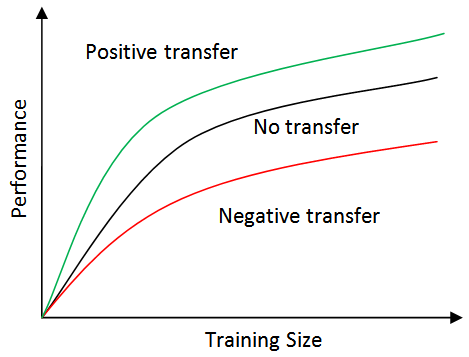
\includegraphics[scale=.5]{fig/negative.png}
%\caption{Positive transfer VS Negative transfer. %Relying on unrelated prior knowledge too much could %lead to negative transfer.}\label{fig:neg}
%\end{figure}
\begin{figure}
\centering
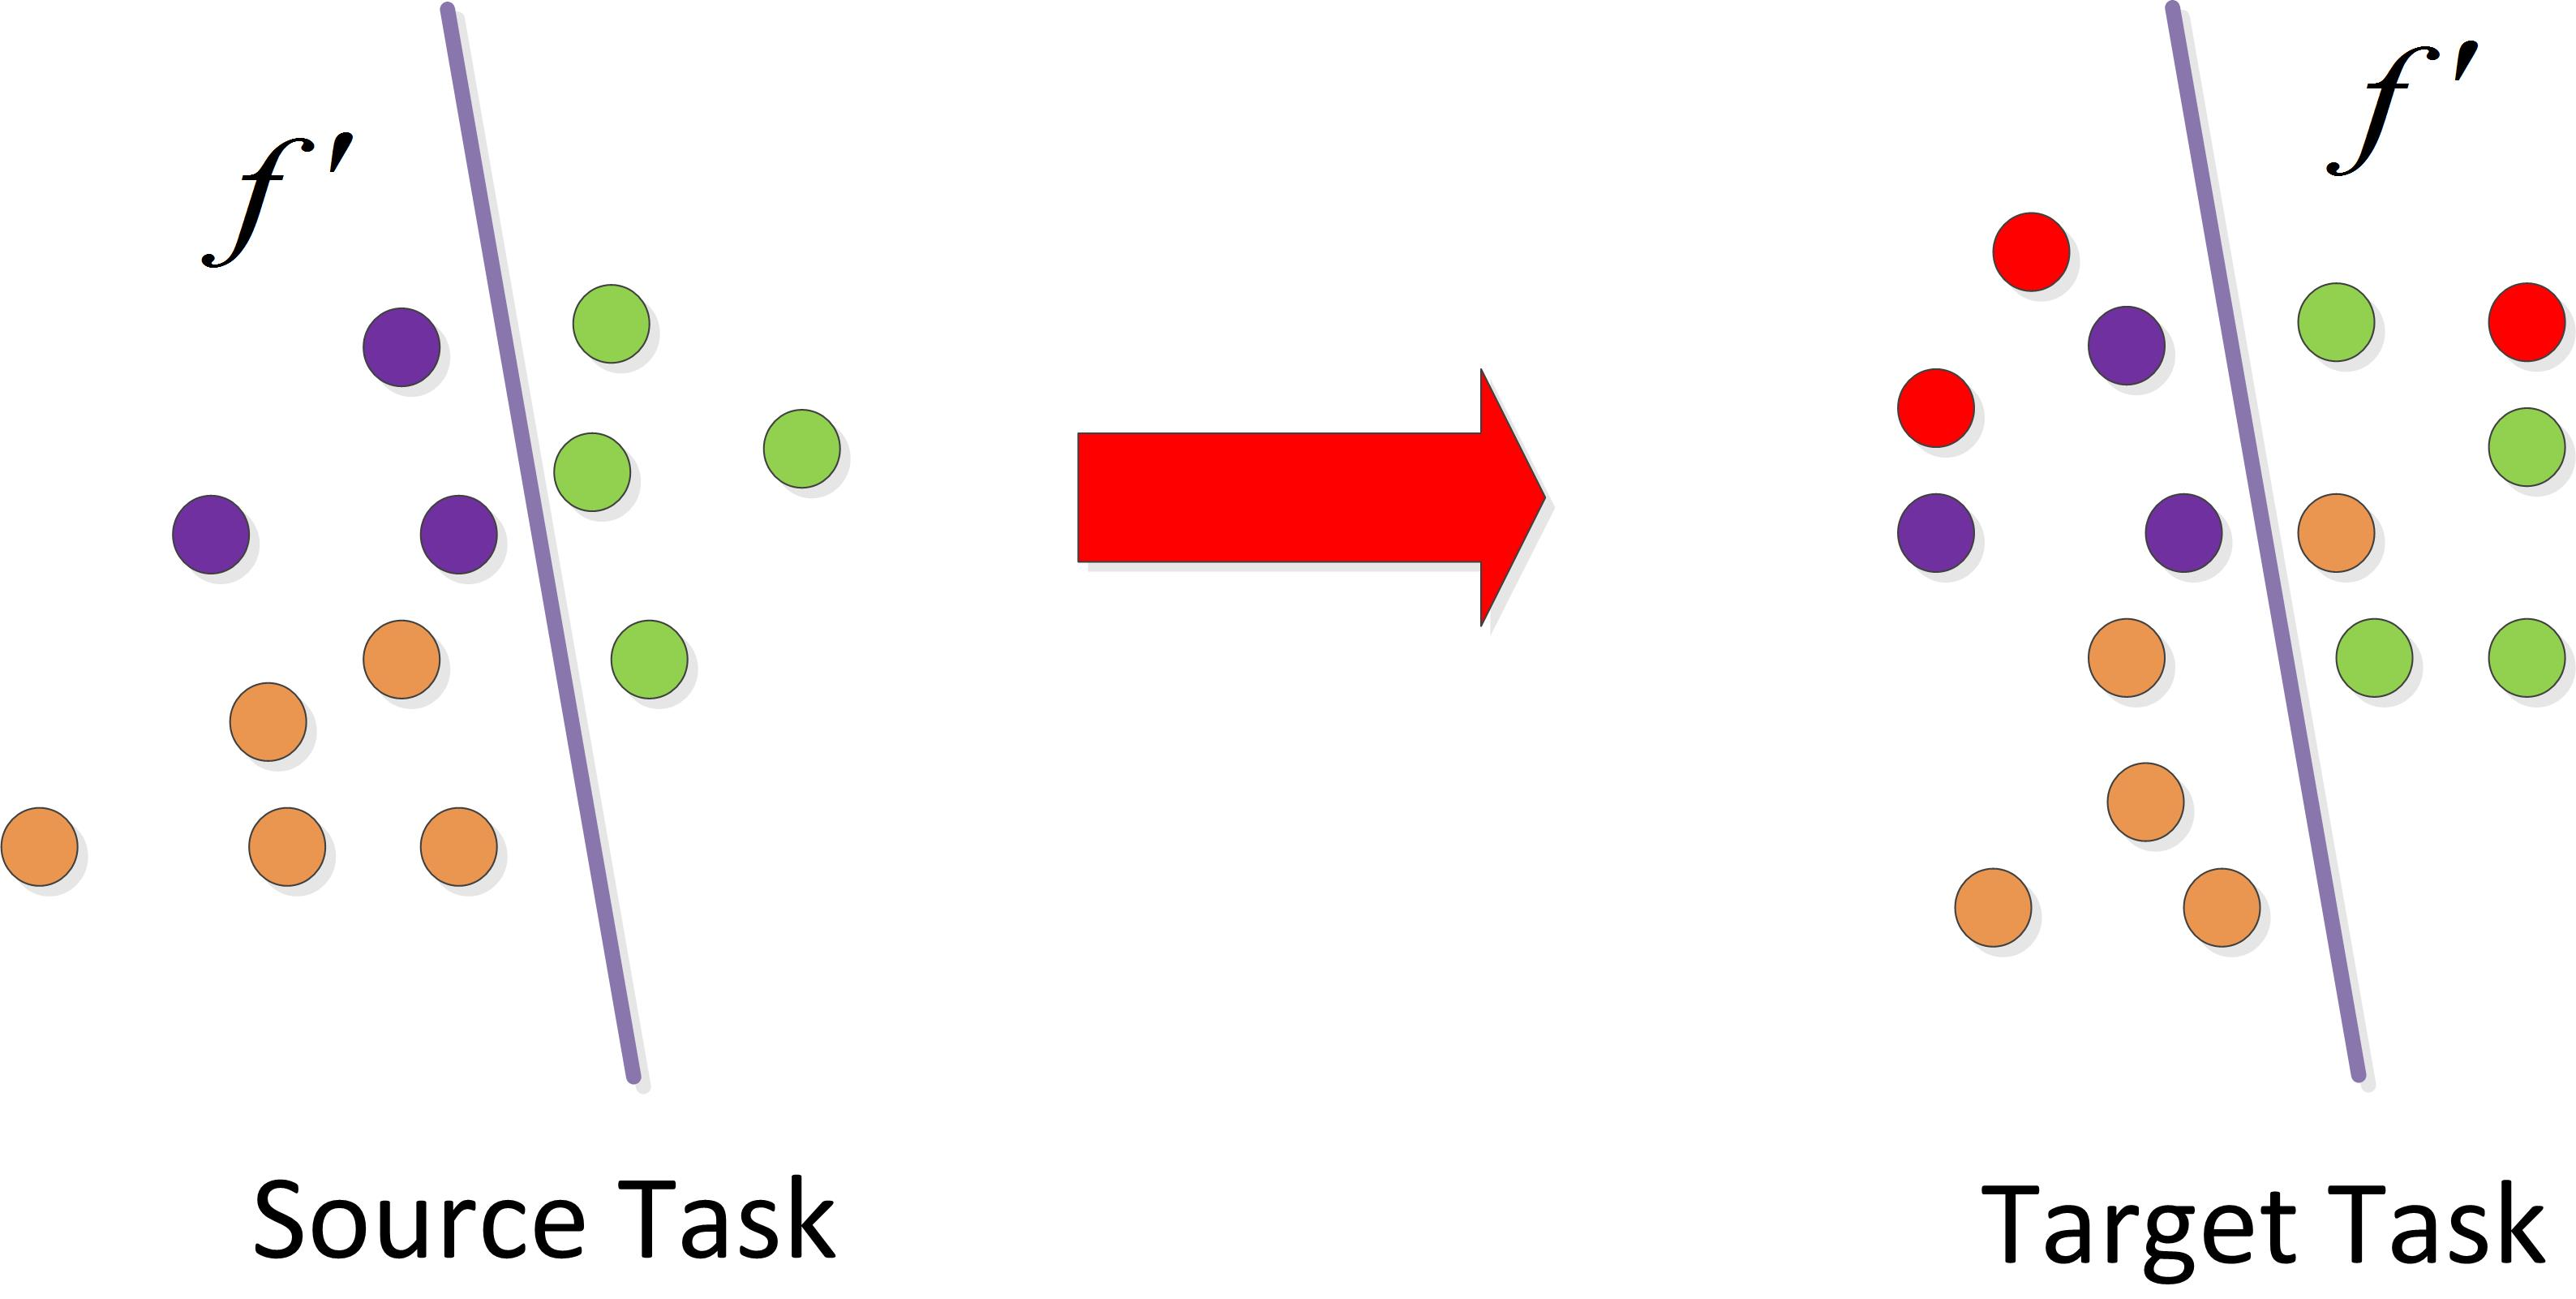
\includegraphics[scale=.4]{fig/domain.jpg}
\caption{Negative transfer happens when we transfer prior hypothesis $f'$ to target one. Points with different color represent different categories. The data distribution would change even for identical categories in different task. The new added category (red points) can also greatly affect the data distribution in target task. }\label{fig:distribution}
\end{figure}
In HTL, a number of empirical works have been attempted with Least Square Support Vector Machine (LS-SVM) \cite{kuzborskij2013stability}. 
The framework of HTL with LS-SVM has two major phrases: (I) Building binary One-Versus-All SVMs with some biased regularization. (II) Estimating transfer parameters with some objective functions.
Following these two phrases, we propose our method, called Safety Multiclass Incremental Transfer Learning (SMITLe), that can both avoid negative transfer and leverage correct hypothesis. In Phrase I, a regularization term adopted from Multi-KT \cite{tommasi2014learning} is used to adapt the $N$ original categories and the new category. As a result, the decision of each binary LS-SVM is the linear combination of the prior hypotheses and empirical knowledge controlled by some transfer parameters. In Phrase II, to measure the transferability of each prior hypothesis, we estimate our transfer parameters using multi-class prediction error based on closed-form leave-one-out (LOO) error for model evaluation.
Then we propose our novel objective function that can balance the weight between the prior hypotheses and empirical knowledge from target task. Experimental results show that SMITLe can achieve better accuracy than other baselines.

The main contributions of this paper include: (1) We propose a novel algorithm SMITLe within the HTL framework that can autonomously utilize the prior hypotheses to prevent negative transfer. (2) We also show that SMITLe can obtain the optimal solution at the rate of $O(\frac{\log(t)}{t})$ where $t$ is training iteration.

The rest of this paper is organized as follow.
In Section \ref{sec:prob}, we introduce the biased regularization terms of our problem for phrase 1 of HTL. Then, we propose a novel objective function for transfer parameter estimation, called SMITLe in Section \ref{sec:smitle}. We show that the estimated transfer parameter can distinguish the utility of the prior hypothesis and avoid negative transfer autonomously. In Section \ref{sec:exp}, we show the performance comparison between SMITLe and other baselines on a variety of experiments on AwA and Caltech datasets in three different scenarios.


%\section{Related Work}\label{sec:work}
%The motivation of transfer knowledge between different domains is to apply the previous information from the source domain to the target one, assuming that there exists certain relationship, explicit or implicit, between the  feature space of these two domains \cite{pan2010survey}. Technically, previous work can be concluded into solving the following three issues: what, how and when to transfer \cite{tommasi2014learning}.


\textbf{What to transfer.} Previous work tried to answer this question from three different aspects: selecting transferable instances, learning transferable feature representations and transferable model parameters. Instance-based transfer learning assume that part of the instances in the source domain could be re-used to benefit the learning for the target domain. Lim et al. proposed a method of augmenting the training data by borrowing data from other classes for object detection \cite{lim2012transfer}. Learning transferable features means to learn common feature that can alleviate the bias of data distribution in target domain. Recently, Long et al. proposed a method that can learn transferable features with deep neural network and showed some impressive results on the  benchmarks \cite{LongICML15}. Parameter transfer
approach assumes that the parameters of the model for the source task can be transfered to the target task. Yang et al. proposed Adaptive SVMs by transferring parameters by incorporating the auxiliary classifier trained from source domain \cite{yang2007cross}. On top of Yang's work, Ayatar et al. proposed PMT-SVM that can determine the transfer regularizer according to the target data automatically \cite{aytar2011tabula}. Tommasi et al. proposed Multi-KT that can utilize the parameters from multiple source models for the target classes  \cite{tommasi2014learning}.
Kuzborskij et al. proposed a similar method to learn new categories by leveraging over the known source \cite{kuzborskij2013n}.

\textbf{When and how to transfer.} The question \textit{when to transfer} arises when we want to know if the information acquired from previous task is relevant to the new one (i.e. in what situation, knowledge should not be transfered). 
\textit{How to transfer} the prior knowledge effectively should be carefully designed to prevent inefficient and negative transfer. Some previous work consists in using generative probabilistic method \cite{davis2009deep} \cite{wang2014active} \cite{zhou2014multi}.  Bayesian learning methods can predict the target domain by combining the prior source distribution to generate a posterior distribution. Alternatively, some previous max margin methods show that it is possible to learn from a few examples by minimizing the  Leave-One-Out (LOO) error for the training model \cite{kuzborskij2013n} \cite{tommasi2010safety}. Previous work shows that there is a closed-form implementation of LOO cross-validation that can generate unbiased model estimation for LS-SVM \cite{cawley2006leave}.

Our work correspond to the context above. In this paper, we propose SMITLe based on parameter transfer approach with LS-SVM. We address our work on how to prevent negative transfer when the source data is not accessible. Compared to other works, we propose a novel strongly convex objective function for transfer parameters estimation. We show that SMITLe can converge at the rate of $O(\frac{\log(t)}{t})$. 
By optimizing this objective function, SMITLe can autonomously adjust the transfer parameters for different prior knowledge. We theoretically and empirically show that, without any data distribution assumption, the superior bound of the training loss for SMITLe is the loss of a method learning directly (i.e. without using any prior knowledge). Experiment results show that when the prior knowledge hurts the transfer procedure, SMITLe can avoid negative transfer by ignoring the unrelated prior knowledge autonomously. Extensive experiments also show that when the prior knowledge is very related (positive transfer), our method can outperform other methods by exploiting the prior knowledge greatly.


\section{Biased Regularization}\label{sec:prob}
 %In order to solve our new task, we would expect our classifier to get improved performance with respect to
%\begin{itemize}
%\item Exploiting knowledge from related source models. If these two tasks are related, SMITLe should transfer the prior knowledge aggressively. In some cases where the prior knowledge is very related and training size of the target task is small, the final decision of the classifier could be mainly rely on the decision from the source models.
%\item Disposing unrelated knowledge. If the knowledge between these two tasks is unrelated, the algorithm should be able to distinguish and dispose the unrelated knowledge autonomously. In the worst case, none of the prior knowledge is related and SMITLe should show similar performance as the model trained merely from target data.
%\end{itemize}

%In this paper, we use LS-SVM as the classifier for the multi-class incremental transfer problem. In the following, we briefly introduce the mathematical setting of our problem.

In this section, we focus on the Phrase I of HTL and introduce our biased regularization for binary LS-SVM for our problem. We use multi-source transfer strategy to generate our biased regularization. As a result, the decision of each binary LS-SVM is the linear combination of the knowledge from both target task and source hypotheses controlled by certain transfer parameters.

We define our task in the following way: assume that, for our $(N+1)$-category target task, ${x} \in \mathcal{X}$ and ${y} \in Y=\left\{1,2,...,N+1\right\}$ are the input vector and output for the learning task respectively. Meanwhile, we have a set of binary linear classifiers (hypotheses) $f'_n(x)=\phi(x)w_n'+b_n'$, for $n=1,...,N$ trained from an unknown distribution with One-Versus-All (OVA) strategy.  Now we want to learn a set of classifiers $f_n(x)=\phi(x)w_n+b_n, n=1,...,N+1$ for our new task. The example $x$ is assigned to the category $j$ if $j \equiv \arg {\max _{n = 1,...,N+1}}\left\{{f_n}(x)\right\}$. From previous works of HTL, the solution of the parameters $(w_n,b_n)$, for each binary LS-SVM, can be found by solving the following optimization problem:
\begin{equation*}
\begin{aligned}
\textbf{min} && R({w_n,W'}) + \frac{C}{2}\sum\limits_i^l {({Y_{i,n}} - \phi ({x_i}){w_n} - {b_n})^2} \\
\end{aligned}
\end{equation*}
Here, $W'=\{w_1',w_2',...,w_n'\}$. $R({w_n,W'})$ is the regularization term to guarantee good transfer performance and avoid overfitting. $\mathbf{Y}$ is a encoded label matrix so that $Y_{in}=1$ if $y_i=n$ and $-1$ otherwise.


Now our task can be divided into two separate part: learning the $(N+1)_{th}$ new category and $N$ overlapped categories.

For the new added category, it is very difficult to identify the utility of the hypothesis of a single category in source task, therefore, we use multi-source transfer strategy, adopted from Multi-KT \cite{tommasi2014learning}, to leverage hypotheses from multiple sources. As a result, regularization term $R(w_{N+1},W')$ can be written as:
\begin{equation}
\begin{aligned}
R(w_{N+1},W')= \frac{1}{2}{\left\| {{w_{N + 1}} - \sum\limits_{k = 1}^N {w{'_k}{\beta _k}} } \right\|^2} 
\end{aligned}\label{eq:multi}
\end{equation}
We can interpret the biased regularization in the following way. Let $w_{N+1} = w_{N+1}''+\sum\limits{\beta _kw'_k}$ (See Figure \ref{fig:combine}). Therefore, we have:
\begin{equation*}
w_{N+1}\phi(x)=w_{N+1}''\phi(x)+\sum\limits{\beta _kw'_k\phi(x)}
\end{equation*}

\begin{figure}
\centering
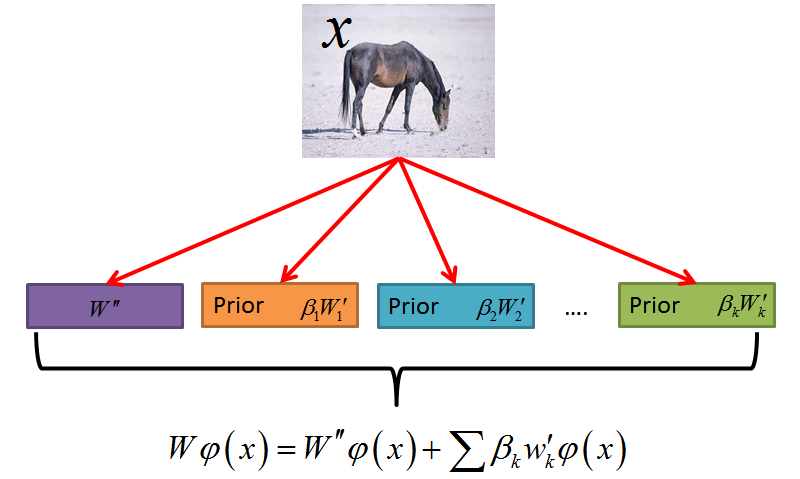
\includegraphics[scale=0.25]{fig/combine.png}
\caption{The final decision function value of a binary SVM can be get by combining the prior and empirical knowledge.}\label{fig:combine}
\end{figure}
Here, we call $\beta$ the transfer parameter. For any fixed value of $\beta$, regularizing $w_n$ is equivalent to regularize $w_{N+1}''$, i.e. $(w_{N+1}-\sum\limits{\beta _kw'_k})$. The decision of each binary SVM model is made by combining the decision from target task $w_{N+1}''\phi(x)$ and source hypotheses $w'_k\phi(x)$ controlled by the transfer parameter. The amount of transfered knowledge has a positive correlation to the value of $\beta$.

However, for the original $N$ categories, we already have their corresponding source category hypotheses and thus, their regularization term can be written as:
\begin{equation}\label{eq:asvm}
\begin{aligned}
R(w_n,w_n')= \frac{1}{2}{{{\left\| {{w_n} - {\gamma _n}{{w'}_n}} \right\|}^2}}  
\end{aligned}
\end{equation}
As we can see that the regularization term \eqref{eq:asvm} is a special case of \eqref{eq:multi} where only one $\beta_k$ is none-zero. 

Combining these two together, our multi-class incremental transfer problem can be solved by optimizing the following objective function:
\begin{equation}
\begin{aligned}
\textbf{min}\qquad {} & \frac{1}{2}\sum\limits_{n = 1}^N {{{\left\| {{w_n} - {\gamma _n}{{w'}_n}} \right\|}^2}}  + \frac{1}{2}{\left\| {{w_{N + 1}} - \sum\limits_{k = 1}^N {w{'_k}{\beta _k}} } \right\|^2}\\& +\frac{C}{2}\sum\limits_{n = 1}^{N + 1} {\sum\limits_{i = 1}^l {e_{i,n}^2} }  \\
\textbf{s.t.}\qquad {} &{e_{i,n}} = {Y_{in}} - \phi ({x_i}){w_n} - {b_n}, \quad n \in \{1,...,N+1\}
\end{aligned}\label{eq:opt}
\end{equation}

The optimal solution to  Eq. (\ref{eq:opt}) is:
\begin{equation}\label{eq:solu}
\begin{aligned}
{w_n}&= {\gamma _n}{{w'}_n} + \sum\limits_i^l {{\alpha _{in}}{\phi(x_i)}} ,{n = 1,...,N}\\
{w_{N + 1}}&= \sum\limits_k^N {{\beta _k}{{w'}_k}}  + \sum\limits_i^l {{\alpha _{i(N + 1)}}{\phi(x_i)}} 
\end{aligned}
\end{equation}
Here $\alpha_{ij}$ is the element $(i,j)$ in $\boldsymbol{\alpha}$. 

Let $K(X,X)$ be the kernel matrix and
\begin{equation}\label{eq:linear}
\psi=\left[ {\begin{array}{*{20}{c}}
{K(X,X) + \frac{1}{C}{\rm{I}}}&\mathbf{1}\\
\mathbf{1^T}&0
\end{array}} \right]
\end{equation}

\begin{equation}
\begin{array}{c}
 {\psi}\left[ {\begin{array}{*{20}{c}}
{\boldsymbol{\alpha} '}\\
{\boldsymbol{b}'}
\end{array}} \right] = \left[ {\begin{array}{*{20}{c}}
Y\\
0
\end{array}} \right], \quad
{\psi}\left[ {\begin{array}{*{20}{c}}
{\boldsymbol{\alpha} ''}\\
{\boldsymbol{b}''}
\end{array}} \right] = \left[ {\begin{array}{*{20}{c}}
{X{{\left( {W'} \right)}^T}}\\
0
\end{array}} \right]
\end{array}
\end{equation}
We have:
\begin{equation}\label{eq:solution}
 \boldsymbol{\alpha}  = \boldsymbol{\alpha} ' - \left[ {\begin{array}{*{20}{c}}
 {\boldsymbol{\alpha} ''\boldsymbol{d_{\gamma}}}&{{\boldsymbol{\alpha} ''\boldsymbol{\beta ^T}}}
 \end{array}} \right]
\end{equation}
Here $\boldsymbol{d_{\gamma}}$ is a diagonal matrix with $\{\gamma_i\}_{i=1,...,N}$ in its main diagonal. From Eq. (\ref{eq:solution}) we can see that, the solution of Eq. (\ref{eq:opt}) is completed once $\boldsymbol{\gamma}$ and $\boldsymbol{\beta}$ are set.



\section{SMITLe}\label{sec:smitle}
In this section, we focus on the Phrase II of HTL, to estimate the transfer parameter in our task. We introduce an algorithm, called SMITLe, that can effectively estimate unbiased transfer parameter from a small training set. % In SMITLe, we first use unbiased LOO error for model evaluation. Then we propose a novel objective function for transfer parameter optimization. We use sub-gradient descent for optimization and provide some theoretical analysis of the performance for SMITLe.

\subsection{Multi-class Prediction Loss with LOO}
%\hl{In this part, we introduce our method to estimate proper $\boldsymbol{\gamma}$ and $\boldsymbol{\beta}$ that can prevent negative transfer. We use closed-form LOO error to evaluate the performance of SMITLe for multi-class classification.  and optimize $\boldsymbol{\gamma}$ and $\boldsymbol{\beta}$ with our novel objective function to prevent negative transfer.}

From Phrase I, we can see that the amount of knowledge transferred is determined by the transfer parameter $\boldsymbol{\gamma}$ and $\boldsymbol{\beta}$. Generally, we would like to reduce the amount of transfer from the prior hypotheses when they are incorrect. Meanwhile, for those correct ones, aggressively increasing the amount of transfer can boost the performance for the target problem. Once we fix the value of $\boldsymbol{\gamma}$ and $\boldsymbol{\beta}$, our task can be directly solved.

To evaluate different settings of $\boldsymbol{\gamma}$ and $\boldsymbol{\beta}$, we have to their cross-validation error iteratively. In this paper, we choose the Leave-One-Out (LOO) cross-validation error as the evaluation criterion. We choose it for the following two reasons: (1) It is proven that LOO error has a low bias on small training data regime \cite{kuzborskij2013stability}. (2) Moreover, it is exhausted to really perform cross-validations and compare the results for each setting of $(\gamma,\beta)$. An important advantage of choosing LS-SVM over the other model is that we can obtain unbiased LOO error in closed form without really performing it. 

The unbiased LOO estimation for sample $x_i$ can be written as \cite{cawley2006leave}:
\begin{equation}
{\hat Y_{i,n}} = {Y_{i,n}} - \frac{{{\alpha _{in}}}}{{\psi_{ii}^{ - 1}}}\quad {\text{for}}\quad n = 1,...,N + 1
\end{equation}
Here $\psi^{-1}$ is the inverse of matrix $\psi$ and  $\psi_{ii}^{-1}$ is the $ith$ diagonal element of $\psi^{-1}$. 

Let us call $\xi_i$ the multi-class prediction error for example $x_i$. $\xi_i$ can be defined as \cite{crammer2002algorithmic}:
\begin{equation}\label{eq:train_loss}
\xi_i(\gamma,\beta) = \mathop {\max }\limits_{n \in \left\lbrace 1,...,N+1 \right\rbrace } {\left[ {1 - {\varepsilon _{n{y_i}}} + {{\hat Y}_{in}}\left( {\gamma ,\beta } \right) - {{\hat Y}_{i{y_i}}}\left( {\gamma ,\beta } \right)} \right]}
\end{equation}
Where $\varepsilon _{n{y_i}}=1$ if $n=y_i$ and 0 otherwise. The intuition behind this loss function is to enforce the distance between the true class and other classes to be at least 1. 

Now, we already have an effective way to measure the performance of different settings of $\boldsymbol{\gamma}$ and $\boldsymbol{\beta}$ for our task. In the next part, we introduce how we optimize these parameters.
\subsection{Loss Function of SMITLe}
In this part, we propose a novel objective function according to our multi-class prediction loss function for transfer parameter estimation. We show that we can effectively obtain the optimal $\boldsymbol{\gamma}$ and $\boldsymbol{\beta}$ that is resistant to negative transfer. 
 
From \eqref{eq:train_loss} we can see that, different from the binary scenario where 0 is used as the hard threshold to distinguish the two classes, our multi-class loss only depends on the gap between the decision function value of the correct label ($\hat Y_{y_i}$) and the maximum among the decision function value of the other labels ${{\hat Y}_{in}}(n \ne y_i)$. To reduce $\xi_i$ for a specific example $x_i$, we only have to increase the gap between ${{\hat Y}_{in}(n \ne y_i)}$ and ${{\hat Y}_{i{y_i}}}$. 

As we mentioned before, the amount of knowledge transfered is positively correlated to the value of transfer parameter. 
When the prior hypotheses are correct, we have $w'_{y_i}\phi ({x_i})> w'_{n}\phi ({x_i})$. If $\xi_i>0$, increasing the transfer parameters can reduce the gap between ${\hat Y_{y_i}}$ and ${{\hat Y}_{in}(n \ne y_i)}$, leading to smaller $\xi_i$. When the prior hypotheses are incorrect and $\xi_i>0$, there exists a $j(j\ne y_i)$ such that $w'_{y_i}\phi ({x_i})<w'_{j}\phi ({x_i})$. Thus, reducing the transfer parameter can eventually reduce $\xi_i$.

Instead of optimize $\xi_i$ directly, we add two extra regularization terms for $\boldsymbol{\gamma}$ and $\boldsymbol{\beta}$. Then we define our objective function as:
\begin{equation}\label{eq:loss}
\begin{aligned}
& \textbf{min}
& & \frac{{{\lambda _1}}}{2}\sum\limits_{n = 1}^N {{{\left\| {{\gamma _n}} \right\|}^2}}  + \frac{{{\lambda _2}}}{2}\sum\limits_{n = 1}^N {{{\left\| {{\beta _n}} \right\|}^2}}  + \sum\limits_{i = 1}^l {{\xi _i}}   \\
& \textbf{s.t.}
& & 1 - {\varepsilon _{n{y_i}}} + {\hat Y_{in}}\left( {\gamma ,\beta } \right) - {\hat Y_{i{y_i}}}\left( {\gamma ,\beta } \right) \le {\xi_i};\\
& & &\lambda_1,\lambda_2 \ge 0
\end{aligned}
\end{equation}

Here $\lambda_1$ and $\lambda_2$ are two regularization parameters to prevent negative transfer. 
By adding these two regularization terms, the objective function \eqref{eq:loss} turns to be strongly convex. Therefore, its strongly convex property guarantees that SMITLe can converge at the rate of $O(\frac{\log(t)}{t})$ (see proof in Appendix \ref{appd:convg}).

From the objective function above we can see that, for certain $\lambda_1$ and $\lambda_2$, when the prior hypotheses are incorrect and harmful, decreasing $\boldsymbol{\gamma}$ and $\boldsymbol{\beta}$ leads to smaller loss from both regularization and multi-class prediction error for target task. Moreover, we also prove that with optimal $\boldsymbol{\gamma}$ and $\boldsymbol{\beta}$ from this objective function, SMITLe can actually avoid negative transfer (see Appendix \ref{appd:proof}). On the other hand, if the prior hypotheses are incorrect, even though, increasing $\boldsymbol{\gamma}$ and $\boldsymbol{\beta}$ leads to larger regularization loss, it also leads to smaller multi-class prediction error on the target problem. Therefore, the algorithm compromises between them.
 
\subsection{Optimizing $\boldsymbol{\gamma}$ and $\boldsymbol{\beta}$}
By adding a dual set of variables in objective function \eqref{eq:loss}, one for each constraint in, we get the Lagrangian of the optimization problem:
\begin{equation}\label{eq:dual}
\begin{aligned}
 &L\left( {\gamma ,\beta ,\xi ,\eta } \right) =
 \frac{{{\lambda _1}}}{2}\sum\limits_{n = 1}^N {{{\left\| {{\gamma _n}} \right\|}^2}}  + \frac{{{\lambda _2}}}{2}\sum\limits_{n = 1}^N {{{\left\| {{\beta _n}} \right\|}^2}}  + \sum\limits_{i = 1}^l {{\xi _i}} \\
   &+ \sum\limits_{i,n} {{\eta _{i,n}}\left[ {1 - {\varepsilon _{n{y_i}}} + {{\hat Y}_{in}}\left( {\gamma ,\beta } \right) - {{\hat Y}_{i{y_i}}}\left( {\gamma ,\beta } \right) - {\xi _i}} \right]}  \\
 &\textbf{s.t.} \quad  \forall i,n \quad {} {\eta _{i,n}} \ge 0
\end{aligned}
\end{equation}

To obtain the optimal values for the problem above, we introduce our method using sub-gradient descent \cite{BoydCO} and summarize it in Algorithm. \ref{alg:1}. 
\begin{algorithm}\label{alg:1}
       \caption{SMITLe optimization}\label{alg:1}
        \begin{algorithmic}[1]
            \REQUIRE $\psi,\alpha',\alpha'',T,\psi$,
            \ENSURE $\gamma=\left\{\gamma^1,...,\gamma^n\right\}, \beta$
            \STATE $\beta^0\leftarrow 0, \gamma^0 \leftarrow 1$
            \FOR {$t=1$ to $T$}
                \STATE $\hat Y \leftarrow Y - {\left( {\psi \circ I} \right)^{ - 1}}\left( {\alpha' - \left[ {\begin{array}{*{20}{c}}
{\alpha''d_\gamma }&{\alpha''\beta^T }
\end{array}} \right]} \right)$
                \STATE ${\Delta _\gamma }=0, {\Delta _\beta }=0$
                \FOR {$i=1$ to $l$}
                	\STATE ${\Delta _\gamma }\leftarrow {\Delta _\gamma }+\lambda_1\gamma$    , 
                	 ${\Delta _\beta }\leftarrow {\Delta _\beta }+\lambda_2\beta$
                	\FOR {$r=1$ to $N+1$}
	                    \STATE $l_{ir} = 1 - {\varepsilon _{{y_i}r}} + {\hat Y_{ir}} - {\hat Y_{i{y_i}}}$
	                    \IF{$l_{ir}>0$}
	                        \IF {$y_i,r \in \{1,...,N\}$}
	                            \STATE $\Delta _\gamma^{{y_i}} \leftarrow \Delta _\gamma^{{y_i}} - \frac{{{\alpha''_{i{y_i}}}}}{{{\psi^{-1}_{ii}}}}$   ,   
	                             $\Delta _\gamma^{{r}} \leftarrow \Delta _\gamma^{{r}} + \frac{{{\alpha''_{i{r}}}}}{{{\psi^{-1}_{ii}}}}$%
	                        \ELSIF {$y_i=N+1$}
	                            \STATE ${\Delta _\beta } \leftarrow {\Delta _\beta } - \frac{{{\alpha''_i}}}{{{\psi^{-1}_{ii}}}}$     ,
	                              $\Delta _\gamma^{{r}} \leftarrow \Delta _\gamma^{{r}} + \frac{{{\alpha''_{i{r}}}}}{{{\psi^{-1}_{ii}}}}$%
	                        \ELSE
	                            \STATE $\Delta _\gamma^{{y_i}} \leftarrow \Delta _\gamma^{{y_i}} - \frac{{{\alpha''_{i{y_i}}}}}{{{\psi^{-1}_{ii}}}}$      ,
	                            ${\Delta _\beta } \leftarrow {\Delta _\beta } + \frac{{{\alpha''_i}}}{{{\psi^{-1}_{ii}}}}$
	                        \ENDIF
	                    \ENDIF
	                 \ENDFOR %class ends   
                \ENDFOR %examples ends
                \STATE $\beta^t \leftarrow \beta^{(t-1)} - \frac{{{\Delta _\beta }}}{{l \times {t} }}$    ,
                 $\gamma^t  \leftarrow \gamma^{(t-1)}  - \frac{{{\Delta _\gamma }}}{{l\times {t} }}$
             \ENDFOR %iteration ends
        \end{algorithmic}
\end{algorithm}


\section{Experiment}\label{sec:exp}
In this section, we show empirical results of our algorithm on different transferring situations on two datasets: AwA10\footnote{The features of AwA dataset is available from http://attributes.kyb.tuebingen.mpg.de/} \cite{lampert2009learning} and Caltech10\footnote{Images for Caltech is available from http://www.vision.caltech.edu/Image\_Datasets/Caltech256/} \cite{griffin2007caltech}. In real world applications, there are three situations in HTL. The first two extreme cases are all the hypotheses are correct/incorrect. The third one is the intermediate (mixed) case where only part of the hypotheses are correct. We design three sets of experiment, called positive, negative and mixed transfer experiment respectively, based on these 3 situations, comparing our algorithm with the baselines.
\subsection{Dataset}
Caltch10 is a subset of Caltech256. We select the following 10 categories: \textit{bat, bear, dolphin, giraffe, gorilla, horse, leopard, raccoon, skunk, zebra}, containing 1387 images, as our dataset.
AwA10 is a subset of AwA dataset. We choose the identical 10 categories as those in Caltech10 from it, containing 6917 images.

\subsection{Baselines and algorithmic setup}
We compare our algorithm with two kinds of baselines. The first one is methods without leveraging any prior knowledge (no transfer baselines). The second consists of some methods with transfer techniques. 

We select 3 no transfer baselines:
\textbf{No transfer:} LS-SVM trained only on target data. Any transfer algorithm that performs worse than it suffers from negative transfer. \textbf{Batch:} We combined the source and target data, assuming that we have full access to all data, to train the LS-SVM. The result of this baseline might be considered as the best performance achieved when the hypotheses are correct. We only perform this baseline in positive transfer experiment. \textbf{Source+1:} This method only train a new binary LS-SVM for the new category. For the rest of the classes, we use the predictions of the classifiers trained from source data directly. Its performance indicates the correctness of the hypotheses.


We select the 3 HTL methods, {MKTL \cite{jie2011multiclass}}, {MULTI-KT \cite{tommasi2014learning}} and MULTIpLE \cite{kuzborskij2013n}, as our transfer baselines.

%\textbf{MKTL \cite{jie2011multiclass}:} This method uses the output of source models as extra feature inputs and automatically determine from which source models to transfer and how much to transfer.


%\textbf{MULTI-KT \cite{tommasi2014learning}:} This method has similar idea with MKTL. It uses LOO error to determine how much to transfer from source models and convert it into solving the convex optimization problem.

%\textbf{MULTIpLE \cite{kuzborskij2013n}:} The basic setting of this method is similar to ours. It is designed to balance the performance between learning the new category and preserving the model from prior knowledge.

For all the experiments in this section, we adopt the same strategy as \cite{kuzborskij2013n} and \cite{tommasi2014learning}, using kernel averaging \cite{gehler2009feature} to compute the average of RBF kernels over the available features on RBF hyperparameter $\{2^{-5},2^{-4},...,2^8\}$. The penalty parameter $C$ is tuned via cross-validation on $\{10^{-5},10^{-4},...,10^8\}$ and the optimal value is reused for all the algorithms.
Two transfer regularization parameters $\lambda1$ and $\lambda2$ are also set via cross-validation on $\{10^{-3},10^{-2},...,10\}$ respectively.

\subsection{Positive transfer: transferring from correct hypotheses}
In the extreme case, where the hypotheses are correct, the data of the source and target tasks should be drawn from the same distribution. Thus, we perform two experiments under this setting on both AwA and Caltech. For each dataset, we split the data into two sets. One is treated as the source dataset to train the source hypotheses and another is treated as the target dataset for training and testing. We iteratively choose one category as the new category and run the experiment 10 times. Due to space constraint, we only report the average results of the two experiments in Table \ref{tab:C2C} and Table \ref{tab:A2A}. From the results, we can see that SMITLe can achieve high classification accuracy than other baselines in most of the cases.
%in Caltech experiment, our algorithm consistently outperforms all the baselines (even better than Batch method). In AwA dataset, Source+1 outperforms SMITLe when the training size is 5. As we increase the training size, the accuracy of SMITLe increases and outperforms Source+1.

To illustrate the detail performance of our algorithm, we select the experiment result on AwA dataset where the horse is chosen as the new category for further explanation. %In Figure \ref{fig:awa-a}, we show the average performances of different methods on different training size for 10 experiments. We can observe that, as the training size increases, our method can even outperform the batch method.
In Figure \ref{fig:awa} we provide values of $\gamma$ and $\beta$ compared with the parameters of the runner-up transfer algorithm MULTIpLE. We can see that for transfer knowledge between identical categories, MULTIpLE fixes the transfer parameter ($\gamma$) to be 1 while our method sets greater weights for related prior knowledge. By exploiting the positive prior knowledge more aggressively, SMITLe is able to leverage the prior knowledge and outperforms other methods. For the transfer parameter $\beta$ we can see that MULTIpLE tends to keep $\beta$ greater than 0 and SMITLe works more intuitively, setting the positive weight for related categories(giraffe, zebra, and bear etc.) and small or even negative weight for unrelated categories (bat, dolphin, and skunk etc.).


\begin{figure}
\centering
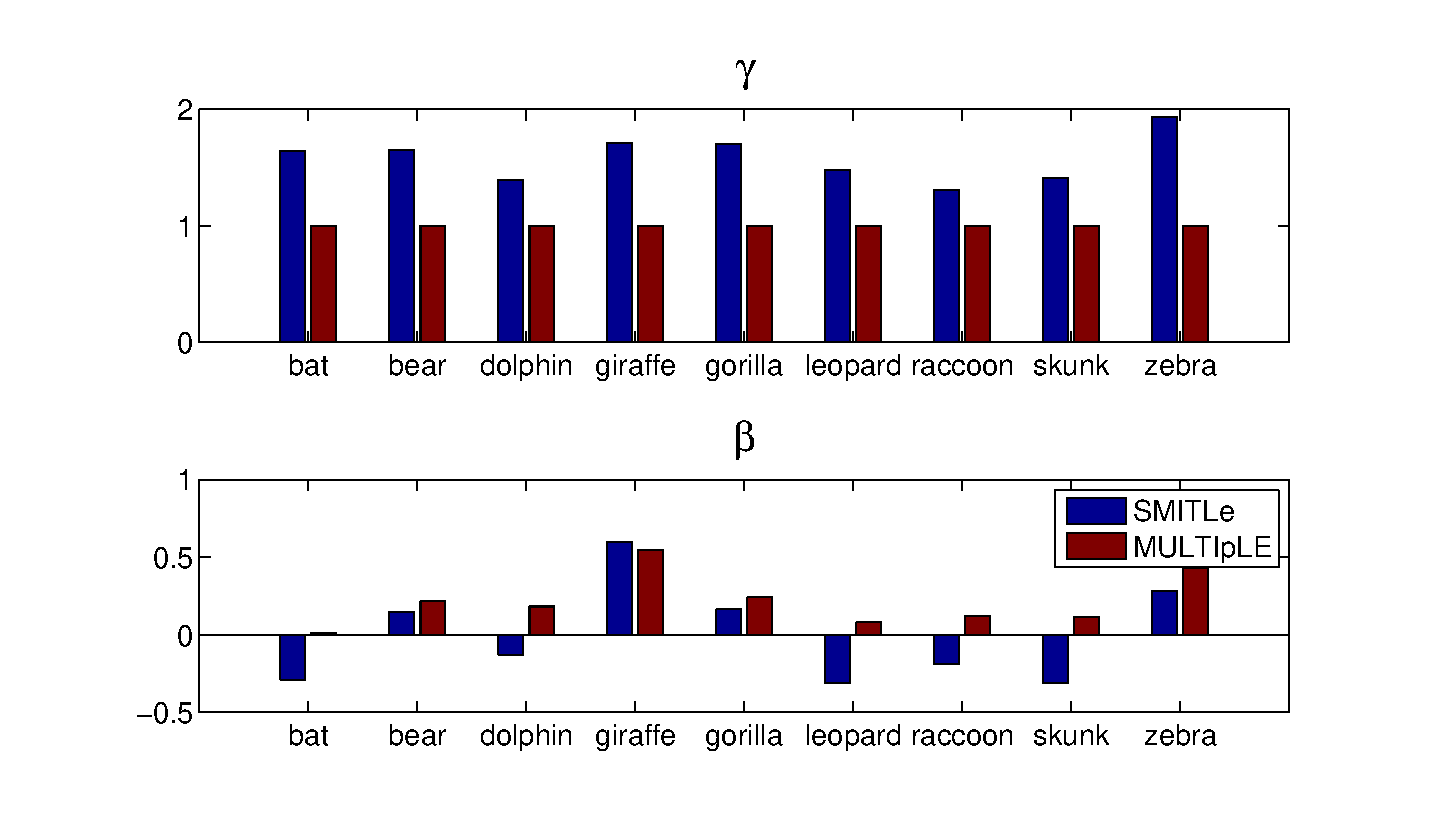
\includegraphics[scale=0.25]{fig/A2A_gama.eps} %\label{fig:awa-b}
\caption{Experiment results for 10 classes, AwA. Horse is used as the new category. We can see that SMITLe tends to more aggressively exploit the related prior knowledge.}
\label{fig:awa}
\end{figure}


\begin{table}[h]
  \centering
  \caption{Average accuracy in percentage across all categories from Caltech to Caltech with different size of the training set in target problem. 30 examples are randomly chosen from each class to train the source classifier and 30 examples from each class are chosen for the test. }
    \begin{tabular}{|c|c|c|c|c|}
    \hline
      \# per category    & 5     & 10    & 15    & 20 \\
    \hline
    No transfer &         27.33  &         31.53  &         35.73  &         38.47  \\
    Source+1    &         43.33  &         43.87   &         44.33  &         44.57   \\
    MKTL        &         38.89  &         43.27   &         45.72  &         47.44   \\
    MULTIKT     &         37.96  &         42.89   &         45.96  &         47.32  \\
    MULTIpLE    &         42.63  &         45.63   &         47.81  &         48.73 \\
    SMITLe        &         \textbf{43.53 }&         \textbf{46.45 } &         \textbf{48.25 } &         \textbf{49.15 } \\
        \hline
    Batch       &         43.77  &         44.73   &         46.67  &         48.00 \\
    \hline
    \end{tabular}%
  \label{tab:C2C}%
\end{table}%

% Table generated by Excel2LaTeX from sheet 'Sheet1'
\begin{table}[h]
  \centering
  \caption{Average accuracy in percentage across all categories from AwA to AwA with different size of the training set in target problem. 50 examples are randomly chosen from each class to train the source classifier and 200 examples from each class are chosen for test.}
    \begin{tabular}{|c|c|c|c|c|}
    \hline
     \# per category    & 5     & 10    & 15    & 20 \\
    \hline
    No transfer &         23.52  &         26.79  &         29.60  &         31.50  \\
    Source+1    &         \textbf{ 39.00 } &         \textbf{ 39.34 } &         39.62 &         39.74  \\
    MKTL        &         31.46  &         34.76  &         37.41  &         38.81  \\
    MULTIKT     &         29.86  &         32.86  &         35.22  &         36.33  \\
    MULTIpLE    &         37.80  &         38.81  &         39.80  &         40.47  \\
    SMITLe        &        37.83  &         { 39.31 } &         \textbf{ 40.37 } &         \textbf{41.09} \\
        \hline
    Batch       &         39.62  &         40.18  &         40.67  &         41.44  \\
    \hline
    \end{tabular}%
  \label{tab:A2A}%
\end{table}%

\subsection{Negative transfer: transferring from incorrect hypotheses}
In this section, we show how our method performs in transferring knowledge between two different datasets, from AwA dataset to Caltech dataset. Following the settings in the previous experiment, the source models are trained from AwA dataset and transferred to Caltech dataset. %We iteratively select one category as the new one, running multiple times to get the average results for all the algorithms. 
We show the average performance of each algorithm in Table \ref{tab:A2C}. We can see that negative transfer does happen when transferring the knowledge from AwA to Caltech for all the algorithms except for ours. From the performance of Source+1, we can see that applying the source hypotheses directly leads to poor performance. We can conclude that even though these two datasets share some categories, the data distribution of the feature representation for the same category is not consistent. 

Still we take the experiment where the horse is considered as the new category to see the detail performance of each algorithm. % and show it in Figure \ref{fig:awa} . 
From here we can see that, not surprisingly, the accuracy of SMITLe shows similar accuracy to the no transfer baseline, while other methods suffer from negative transfer and perform even worse than no transfer baseline. In Figure \ref{fig:a2c} we show the parameters learned for each classes in SMITLe in comparison with MULTIpLE. We can see that when the prior knowledge is unrelated, SMITLe resists utilizing the prior knowledge and, therefore, shows almost identical accuracy to the no transfer baseline.
%\begin{figure*}
%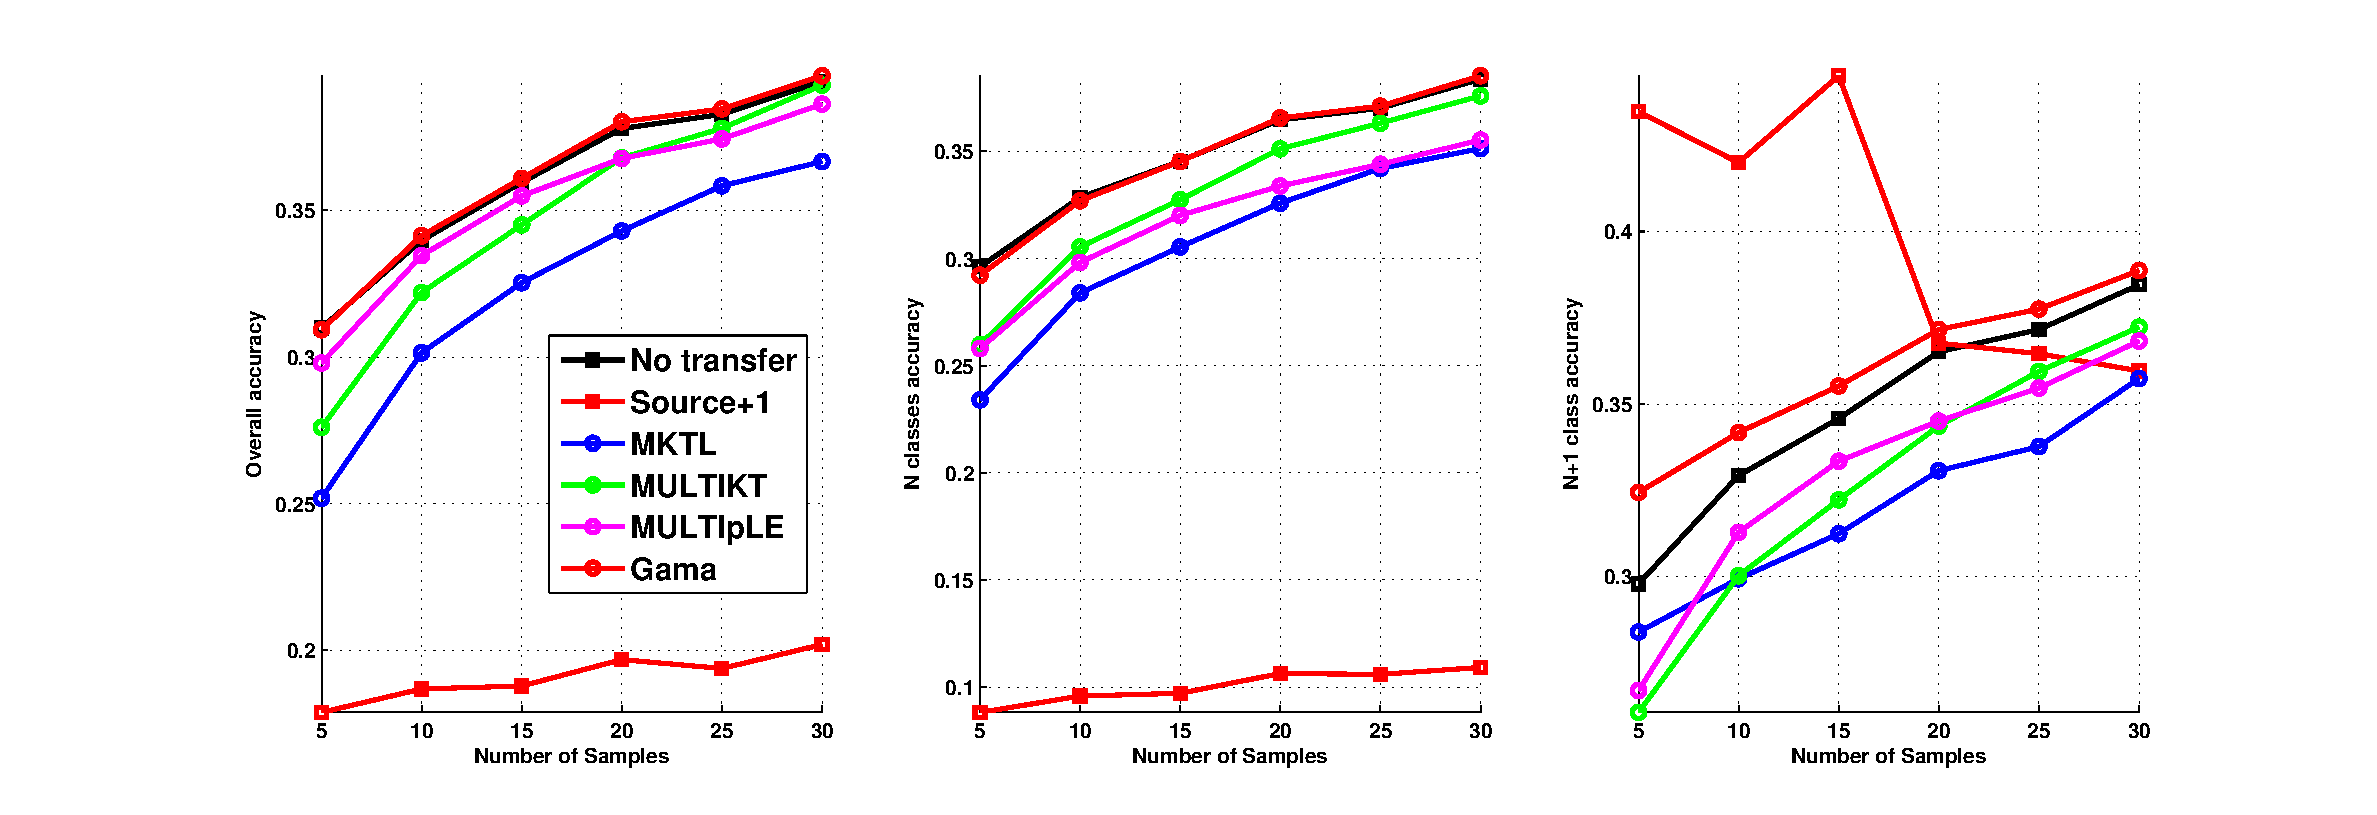
\includegraphics[width=\textwidth,height=5cm]{fig/A2C_RBF_PHOG.eps}
%\caption{Transferring from AwA to Caltech-256.}
%\end{figure*}
% Table generated by Excel2LaTeX from sheet 'Sheet1'

\begin{figure}
    \centering
     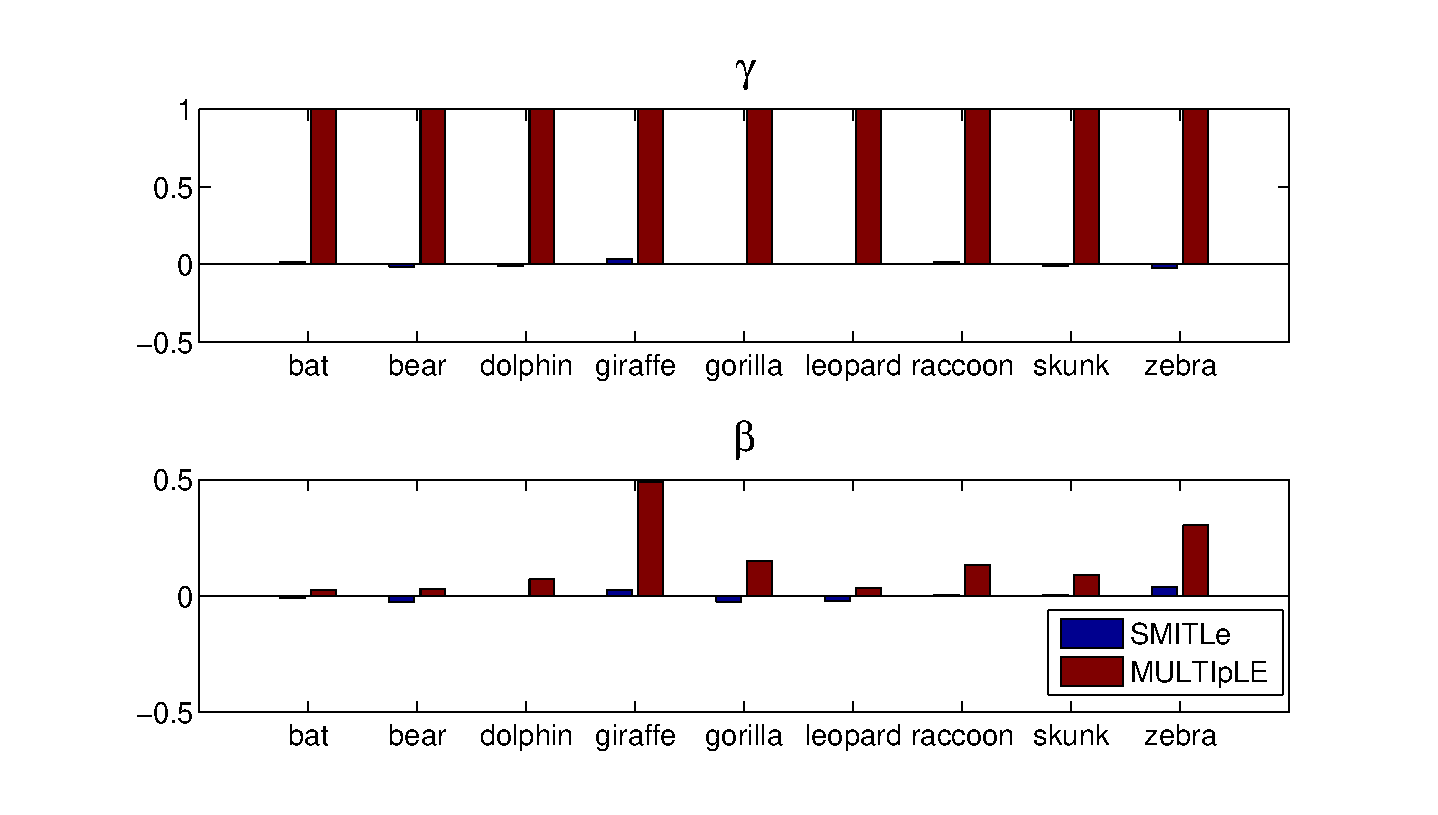
\includegraphics[scale=0.25]{fig/A2C_gama.eps} %\label{fig:a2c-b}
    \caption{Experiment results for 10 classes, AwA. Horse is used as the new category. SMITLe can ignore unrelated prior knowledge.}
    \label{fig:a2c}
\end{figure}


\begin{table}[htbp]
  \centering
  \caption{Average accuracy in percentage across all categories from AwA to Caltech. Examples in AwA are used to train prior models. Different number of training size is randomly selected from Caltech dataset.}
    \begin{tabular}{|c|c|c|c|c|c|}
    \hline
      \# per category           & 5              & 10             & 15             & 20             & 25             \\
    \hline
    No transfer &         \textbf{ 30.99 } &         33.97  &         35.95 &         37.78  &         38.27   \\
    Source+1    &         17.89  &         18.69  &         18.79  &         19.69  &         19.39          \\
    MKTL        &         25.19  &         30.14  &         32.53  &         34.30  &         35.83  \\
    MULTIKT     &         27.60  &         32.19  &         34.51  &         36.78  &         37.79  \\
    MULTIpLE    &         29.79  &         33.45  &         35.49  &         36.77  &         37.43  \\
    SMITLe        &       30.93  &         \textbf{ 34.13 } &         \textbf{  36.09 } &         \textbf{38.01} &         \textbf{38.46} \\
    \hline
    \end{tabular}%
  \label{tab:A2C}%
\end{table}%

\subsection{Transferring from mixed hypotheses}
In real applications, the extreme situation is rare. For most multi-source transfer learning tasks, there should always be some related and useful sources as well as some unrelated ones. In this part, we show how SMITLe performs in the mixed sources.

From negative transfer experiments we see that the knowledge from AwA is unrelated to Caltech and vice versa. To generate mixed sources, we follow the settings in our positive transfer experiment, splitting the AwA dataset into two datasets, and replace the data in some categories in the source dataset with the data of Caltech. 
For example, if the bat is considered as the new category and we have to replace 3 categories, we choose the data from 3 out of 9 categories (10 categories except for bat) in Caltech to replace the source data accordingly. 

We show the performances across all categories of different algorithms in Table \ref{tab:3c} and Table \ref{tab:4c} where 3 and 4 categories in the source data are replaced by the data from Caltech respectively. From the tables, we can see that in almost every case, SMITLe shows improved or equivalent performance than other baselines. %The improved performance of SMITLe is due to the loss function we designed. Compared to other transfer baselines, the loss function Eq. \eqref{eq:loss} is able to control the transfer parameters $\gamma$ and $\beta$ to prevent negative transfer. For other transfer baselines, such as Multi-KT and MULTIpLE, they try to optimize a convex function directly with non-negative L2 ball constraint, which could not be able to handle the negative transfer effectively.

% Table generated by Excel2LaTeX from sheet 'Sheet1'
\begin{table}[htbp]
  \centering
  \caption{Average accuracy in percentage across all categories from AwA to AwA\&Caltech with different size of the training set in target problem. Data of 3 classes in AwA is replaced by the data from Caltech in target problem.}
    \begin{tabular}{|c|c|c|c|c|c|}
    \hline
      \# per category    & 5     & 10    & 15    & 20    & 25 \\
    \hline
    no transfer &         23.99  &         26.24  &         29.02  &         30.05  &         31.18  \\
    source+1 &         25.70  &         26.30  &         26.57  &         26.69  &         26.97  \\
    MKTL  &         25.30  &         27.59  &         30.42  &         31.01  &         31.97  \\
    MultiKT &         25.53  &         27.94  &         30.48  &         31.36  &         32.31  \\
    MULTIpLE &         28.11  &         29.61  &         31.34  &         32.18  &         32.89  \\
    SMITLe &         \textbf{28.75}  &         \textbf{30.48}  &         \textbf{32.30}  &         \textbf{33.06}  &         \textbf{33.71}  \\
    \hline
    \end{tabular}%
  \label{tab:3c}%
\end{table}%



% Table generated by Excel2LaTeX from sheet 'Sheet1'
\begin{table}[htbp]
  \centering
  \caption{Average accuracy in percentage across all categories from AwA to AwA\&Caltech with different size of the training set in target problem. Data of 4 classes in AwA is replaced by the data from Caltech in target problem.}
    \begin{tabular}{|c|c|c|c|c|c|}
    \hline
       \# per category    & 5     & 10    & 15    & 20    & 25 \\
    \hline
    no transfer &         24.02  &         26.25  &         29.06  &         30.07  &         31.20  \\
    source+1 &         23.23  &         23.80  &         24.03  &         24.21  &         24.47  \\
    MKTL  &         24.44  &         26.78  &         29.64  &         30.40  &         31.50  \\
    MultiKT &         24.73  &         27.40  &         29.93  &         30.91  &         31.91  \\
    MULTIpLE &         26.50  &         28.33  &         30.27  &         31.29  &         32.12  \\
    SMITLe &         \textbf{27.20}  &         \textbf{29.33}  &         \textbf{31.40}  &         \textbf{32.31}  &         \textbf{33.11}  \\
    \hline
    \end{tabular}%
  \label{tab:4c}%
\end{table}%


\section{Conclusion}
In this paper, we present a novel method called SMITLe that is able to transfer knowledge across different datasets and learn a new category. Inspired by previous work, SMITLe uses LS-SVM as the basic classification model and LOO for transfer parameter estimation. We demonstrate that SMITLe is able to converge at a logarithmic rate. We also prove that with the transfer parameters optimized by our novel objective function, SMITLe is able to avoid negative transfer which is a general issue for transfer learning. 
We carry out 3 sets of the experiment that our algorithm would face in real world application. 
From the experimental results, we can see SMITLe can consistently outperform other transfer baselines and achieve higher classification accuracy in different scenarios.

\appendix
\section{Convergence Analysis}\label{appd:convg}
%In this part, we show that SMITLe can converge to its optimal solution at the speed of $O(\frac{\log(t)}{t})$ for objective function \eqref{eq:loss}.

%Because $\xi_i(\gamma,\beta)$ is a convex loss function, the primal problem \eqref{eq:loss} becomes the strongly convex problem by adding the L2 regularization terms. Optimizing the strongly convex problem can lead to the following error bound:
%\begin{lemma}[Converge lemma]
%Let $f(\mu)$ be a 1-strongly convex function. Let $\mu_1,...,\mu_t$ be a sequence corresponding to $\mu_t=(\sqrt{\lambda_1}\gamma^t,\sqrt{\lambda_2}\beta^t)$. Let $\Delta_t$ be the sub-gradient for $f(\mu_t)$ and $\mu^*=(\sqrt{\lambda_1}\gamma^*,\sqrt{\lambda_2}\beta^*)$
%\end{lemma}

Let $\mu_1,...,\mu_t$ be a sequence corresponding to $\mu_t=(\sqrt{\lambda_1}\gamma^t,\sqrt{\lambda_2}\beta^t)$. Problem \eqref{eq:loss} can be rewritten as:
\begin{equation*}
J(\mu)=\frac{1}{2}{\left\| \mu  \right\|^2} + \sum\limits_{i = 1}^l {{\xi _i}\left( \mu  \right)} 
\end{equation*}
Let $\Delta_t$ be the sub-gradient for $J(\mu_t)$ and  $\mu^*=(\sqrt{\lambda_1}\gamma^*, \sqrt{\lambda_2}\beta^*)$ be the optimal solution for it. Assume that $\left\| {{\Delta _t}} \right\| \le G$. According to Lemma 1 in \cite{shalev2011pegasos}, we have:
\begin{equation}
J({\mu_t}) - J(\mu^*) \le \frac{{{G^2}}}{{2t}}\left( {1 + \ln \left( t \right)} \right)
\end{equation}
This means that SMITLe converges at the rate of $O(\frac{\log(t)}{t})$.



\section{Proof of avoiding negative transfer}\label{appd:proof}

%From the analysis in Appendix \ref{appd:convg} we can see that, SMITLe can alway converge to its optimal solution with sufficient iterations. We can prove that, with the optimal transfer parameters $\boldsymbol{\gamma}$ and $\boldsymbol{\beta}$, SMITLe can avoid negative transfer.

Assume that $\bar \xi_i$ is the multi-class loss of example $x_i$ without utilizing any prior knowledge, i.e. $\gamma=\beta = \mathbf{0}$. Let $\gamma^*, \beta^*$ be the optimal solution for Eq. \eqref{eq:dual} and $\xi_i^*$ be the multi-class loss with respective to example $x_i$. Then for every example $x_i \in \mathcal{X}$, we have:\[\sum\limits_i {{\xi^* _i}}  \le \sum\limits_i {{{\bar \xi }_i}} \]

\begin{proof}
%For simplification, let $\delta_i=1$ if $i=N+1$ and 0 otherwise, and  ${\theta _{ij}} = {\alpha ''_{ij}}\left( {1 - {\delta _j}} \right)/\psi_{ii}^{ - 1}$. Eq. \eqref{eq:train_loss} can be written as:
%\begin{equation}\label{eq:loss_simple}
%\begin{split}
%{\xi _i}(\gamma ,\beta )=&\mathop {\max }\limits_{n} \bigg \{ {\varepsilon _{n{y_i}}} - 1 + \frac{{\left( {{{\alpha '}_{i{y_i}}} - {{\alpha '}_{in}}} \right)}}{{\psi _{ii}^{ - 1}}} + {\theta _{in}}{\gamma _n} \\
%&- {\theta _{i{y_i}}}{\gamma _{{y_i}}} + \left( {{\delta _n} - {\delta _{{y_i}}}} \right)\sum\limits_k {\frac{{{{\alpha ''}_{ik}}{\beta _k}}}{{\psi_{ii}^{ - 1}}}}  \bigg\}
%\end{split}
%\end{equation}
When $\mathbf{\gamma}=\mathbf{\beta} = \mathbf{0}$, from Eq. \eqref{eq:train_loss} we can get:
\begin{equation*}
{\bar \xi _i} = \mathop {\max }\limits_n \left[ { {\varepsilon _{n{y_i}}}-1 + \frac{{\left( {{{\alpha '}_{i{y_i}}} - {{\alpha '}_{in}}} \right)}}{{\psi _{ii}^{ - 1}}}} \right]
\end{equation*}
%To obtain the optimal value of $\gamma$ and $\beta$, we have to seek the saddle point of the Lagrangian problem in \eqref{eq:dual} by finding the minimum for the prime variables $\left\{ \gamma, \beta, \xi \right\}$ and the maximum for the dual variables $\eta $.
For simplification, let $\delta_i=1$ if $i=N+1$ and 0 otherwise, and  ${\theta _{ij}} = {\alpha ''_{ij}}\left( {1 - {\delta _j}} \right)/\psi_{ii}^{ - 1}$.
To find the minimum of the primal problem, we require:
\begin{equation}
\frac{{\partial L}}{{\partial {\xi _i}}} = 1 - \sum\limits_n {{\eta _{in}}}  = 0 \Rightarrow \sum\limits_n {{\eta _{in}}}  = 1
\end{equation}   
%Similarly, for $\gamma$ and $\beta$, we require:
\begin{eqnarray}\label{eq:opt_gama}
\frac{{\partial L}}{{\partial {\gamma _n}}} = 0  
\Rightarrow  \gamma _n^* = \frac{1}{{{\lambda _1}}}\sum\limits_i {\left( {{\varepsilon _{n{y_i}}} - {\eta _{in}}} \right){\theta _{in}}} 
\end{eqnarray}
%In $=_1$ we use the facts that $\sum_n\eta_{in}=1$ and use $\varepsilon_{ny_i}$ to replace it.
\begin{eqnarray}\label{eq:opt_beta}
\frac{{\partial L}}{{\partial {\beta _n}}}  = 0 
\Rightarrow \beta _n^* = \frac{1}{{{\lambda _2}}}\sum\limits_{i,n} {\frac{{{\eta _{in}}{{\alpha ''}_{in}}}}{{\psi _{ii}^{ - 1}}}\left( {{\delta _{{y_i}}} - {\delta _n}} \right)} 
\end{eqnarray}
As the strong duality holds,the primal and dual objectives coincide. Plug Eq \eqref{eq:opt_gama} and \eqref{eq:opt_beta} into Eq. \eqref{eq:dual}, we have:
\begin{equation*}
\sum\limits_{i,n} {{\eta _{in}}\left[ {1 - {\varepsilon _{n{y_i}}} + {{\hat Y}_{in}}\left( {\gamma^* ,\beta^* } \right) - {{\hat Y}_{i{y_i}}}\left( {\gamma^* ,\beta^* } \right) - {\xi _i^*}} \right]}=0
\end{equation*}
Expand the equation above, we have:
\begin{eqnarray}\nonumber
\sum\limits_{i,n} {{\eta _{in}}\left[ { {\varepsilon _{n,{y_i}}}-1 + \frac{{\left( {{{\alpha '}_{i{y_i}}} - {{\alpha '}_{in}}} \right)}}{{\psi_{ii}^{ - 1}}} - {\xi _i}} \right]} \nonumber\\ 
= {\lambda _1}\sum\limits_r {{{\left\| {\gamma _r^*} \right\|}^2}}  + {\lambda _2}\sum\limits_r {{{\left\| {\beta _r^*} \right\|}^2}}  \ge 0\nonumber
\end{eqnarray}
Rearranging the above, we obtain:
\begin{eqnarray}\label{eq:link1}
\sum\limits_{i,n} {{\eta _{in}}\left[ { {\varepsilon _{n,{y_i}}} -1+ \frac{{\left( {{{\alpha '}_{i{y_i}}} - {{\alpha '}_{in}}} \right)}}{{\psi_{ii}^{ - 1}}}} \right]}  
 \ge \sum\limits_{i,n} {{\eta _{in}}{\xi _i}}  = \sum\limits_i {{\xi _i}} 
\end{eqnarray}
The left-hand side of Inequation \eqref{eq:link1} can be bounded by:
\begin{eqnarray}
&&\sum\limits_{i,n} {{\eta _{in}}\left[ { {\varepsilon _{n{y_i}}}-1 + \frac{{\left( {{{\alpha '}_{i{y_i}}} - {{\alpha '}_{in}}} \right)}}{{\psi_{ii}^{ - 1}}}} \right]} \nonumber\\ &&\le \sum\limits_i {\left( {\sum\limits_n {{\eta _{in}}\mathop {\max }\limits_r \left\{ { {\varepsilon _{r{y_i}}} -1 + \frac{{\left( {{{\alpha '}_{i{y_i}}} - {{\alpha '}_{ir}}} \right)}}{{\psi_{ii}^{ - 1}}}} \right\}} } \right)}  \nonumber\\
&&= \sum\limits_i {\left( {\sum\limits_n {{\eta _{in}}{{\bar \xi }_i}} } \right)}  = \sum\limits_i {\bar \xi_i }
\end{eqnarray}
\end{proof}
%When setting $\gamma=\beta = \mathbf{0}$, we don't utilize any knowledge from previous task (see Eq. \eqref{eq:opt}).
%This suggests that the SMITLe can avoid negative transfer. 
%According to statistic learning theory, we can conclude that, in any case, the superior bound of the risk for SMITLe is the risk of no transfer method, which proves SMITLe can avoid negative transfer.


\bibliographystyle{named}
\bibliography{research}

\end{document}

